\documentclass{article}
\usepackage{amsmath}
\usepackage{amssymb}

\title{无线通信中的快时变信道建模}
\author{}
\date{}

\begin{document}

\maketitle

\begin{center}
\textbf{第十一届华为杯全国研究生数学建模竞赛}
\end{center}

\begin{tabular}{|c|c|}
\hline 符号 & 含义 \\
\hline $v$ & 运动速度 \\
\hline $\hat{x}$ & $x$ 的估计值 \\
\hline $M$ & 基函数阶数 \\
\hline $B_{m}[n]$ & 第 $m$ 个基函数 \\
\hline $L$ & 衰落信道径的数目 \\
\hline $b_{lm}$ & 第 $l$ 径第 $m$ 个基系数 \\
\hline $h_{l}[n]$ & 第 $l$ 径第 $n$ 时刻信道参数 \\
\hline $T_{c}, T_{s}, T$ & 相干时间、采样间隔、信道采样总时间 \\
\hline $f_{s}, f_{c}, f_{m}$ & 信道采样率、载波频率、最大多普勒频移 \\
\hline $N_{\text {tot }}, N$ & 信道数据每径的采样总数、每次估计的样本点数 \\
\hline
\end{tabular}

\begin{center}
\textbf{题目} \quad 无线通信中的快时变信道建模
\end{center}

\begin{abstract}
本文考虑了无线通信中快时变信道的建模问题,基于基扩展模型对多径衰落信道建模,并且分析了运动速度对模型的影响,最后,通过 16QAM 调制解调仿真分析了采用该模型进行信道估计的误比特率性能。

针对问题一,本文建立了快时变信道的基扩展模型,通过分析不同基函数的优缺点,我们选择了适用于多普勒频移的泛化复指数基函数。首先分析了模型参数对模型准确度的影响,结果表明归一化均方误差随基函数阶数增加指数下降,随取样间隔增大而波动。复杂度分析表明复杂度随阶数平方增长,随每次估计样本数线性增加。综合考虑模型准确度与复杂度,我们选择了适当的模型参数,只需要测试 300 个数据点就能计算出 20000 个数据点,归一化均方误差为 $10^{-5}$ 量级。

针对问题二,通过理论计算得出了在不同运动速度下采用问题一中参数最多能估计的样本点数,进一步通过仿真得到误差模值的累积分布函数及统计数据,结果表明速度增加时,相同模型参数预测的准确度大幅下降,需要调整参数来获得较高准确度。

此外,我们基于 Clarke 模型对多径瑞利衰落信道进行仿真,将仿真信道数据用于问题一所建立模型,通过对比仿真信道与实测信道建模误差,两者十分接近,验证了模型能够有效减少测试数据。

针对问题三,经过 16QAM 调制发送信号,通过问题一、二涉及的信道并增加加性高斯白噪声,在接收端进行解调,仿真了不同信噪比条件下,采用 BEM 模型进行信道估计的误比特率。结果表明测试速度越低,误比特率越低。BEM 模型与理想信道估计的性能接近。

关键词 快时变信道 多径衰落 基扩展模型 16QAM 调制 误比特率
\end{abstract}

\tableofcontents

\section{1.问题重述}

宽带移动通信传输正在改变着人们的生活,更为快速和准确的传递信息是其基本需求。据预测,到 2020 年,数以千亿的“物”,包括汽车、计量表、医疗设备和家电等都将连入移动通信网络。复杂多变的移动通信网络连接环境,将对实现高速宽带数据传输提出更高的要求和挑战。其中,高速铁路和高速公路的开通和应用,将使未来移动通信系统面临高速移动环境的挑战。我们需要建立新的数学模型以适应高速移动环境下无线信道的快速变化,从而保证信息传输的速度和质量。

在通信系统中,发送端通过信道传输信号到接收端,在传输过程中,不可避免地要引入干扰噪声。接收端对包含噪声的信号进行合理解码,得到正确的信息,完成信息传输过程,原理用图 1 表示。

\begin{figure}[h]
\centering
\includegraphics[width=0.8\textwidth]{communication_model.png}
\caption{通信模型示意图}
\end{figure}

其相应数学模型可以表示为:

\begin{align*}
        f_m &= \frac{\nu}{c} f_c = \frac{3 \times 10^9 \times 50}{3 \times 10^8} \, \text{Hz} = 500 \, \text{Hz} \\
        T_c &= \frac{1}{f_m} = \frac{1}{500} \, \text{s} = 2 \, \text{ms}
    \end{align*}

从式 (1) 可以看出,在已知接收端信号 \( Y \) 的情况下,要得知发送端的信号 \( X \),还需要知道信道变量 \( H \) 和噪声 \( W \) 的统计特征。\( W \) 可视为加性高斯白噪声 AWGN(Additive White Gaussian Noise),因此通信模型的关键就是对 \( H \) 规律的探索。

在无线信道中,发送和接收之间通常存在多于一条的信号传播路径。多径的存在是因为发射机和接收机之间建筑物和其他物体的反射、绕射、散射等引起的。由于环境的复杂性,信号传播途径也复杂多变,需要对其进行简化和抽象,建立描述、估计信道传播的数学模型。

当信号在无线信道传播时,多径反射和衰减的变化将使信号经历随机波动。无线多径传输系统的时间离散形式的数学表达式为 [1]:

\begin{align*}
    h_l &= (h_l[0], h_l[1], \dots, h_l[N-1])^T, \\
    b_l &= (b_{l0}, b_{l1}, \dots, b_{l(M-1)})^T \\
    B &= \begin{pmatrix}
        B_0[0] & B_1[0] & \cdots & B_{M-1}[0] \\
        B_0[1] & B_1[1] & \cdots & B_{M-1}[1] \\
        \vdots & \vdots & \ddots & \vdots \\
        B_0[N-1] & B_1[N-1] & \cdots & B_{M-1}[N-1]
    \end{pmatrix}
    \tag{8}
\end{align*}

式中 \( L \) 为信道的多径数,\( K \) 为传输信号的长度,\( w(n) \) 可视为 AWGN,\( h_l[n] \) 就是信道参数。由于多径效应的存在,接收端接收到的信号相比于实际发送的信号在时域上被展宽,称为时延扩展。

根据以上的分析可知,如果要准确地从接收端得到发端的信号,必须准确地对无线信道进行估计。

目前,信道的估计方法有多种,其中比较常用的方法是使用训练序列(导频),即在发送端插入训练序列,在接收端根据已知导频可以估计信道。然而,由于信道是时变的,需要周期性地插入训练信号和进行信道参数估计。移动台与基站间的相对运动带来的多普勒效应会使信道特性随时间变化[2][3]。运动速度越快,信道变化越快。在慢衰落信道情况下,使用导频是一种比较准确经济的方法,但在高速运动的快时变信道情况下,就需要频繁地增加训练信号(开销),在接收端增加相同的信道估计次数。由于导频不承载有用信息,过密的导频插入将会占用过多的传输资源,降低有用信息的传输速率。因此,针对快时变信道,有必要找到新的数学模型来估计信道参数,以降低导频的插入频率,提高有用信息的传输速率。

为了减少快时变信道的估计负荷,当前研究热点之一在于寻找可分辨路径的各个抽样值在块传输时间内的相关性,这种相关性使得估计负荷的减少成为可能。基扩展模型主要是利用有限个基函数的线性组合来描述一定时间内的时变信道,可以模拟有多普勒效应的快时变信道,从而减少信道参数直接估计的次数。因此,针对快时变信道,基扩展模型的引入具有十分重要的意义。

本论文将基于基扩展模型研究如下三个问题:

问题一:基扩展模型建立及其准确度、复杂度分析

根据数据文件 1 给出的某信道测试参数(运动速度 $180\mathrm{Km/h}$,载波频率 $3\mathrm{GHz}$,信道采样频率 $200\mathrm{KHz}$),建立数学模型。在保持一定的准确度的情况下,把测试数据中的部分数据通过所建模型计算获得,从而减少实际数据的测试量。用图表方式展示原始数据与计算结果的误差,并分析模型所用算法的复杂度。

问题二:多径时变信道下的基扩展模型分析及验证

\paragraph{问题 2.1 运动速度对基扩展模型准确度的影响规律}

多普勒效应引起信道的变化,在载波频率一定的情况下,变化的程度与相对速度有关[3][4]。数据文件 2、3、4 分别是载波频率为 $3\mathrm{GHz}$ 时,信道在不同速度 $90\mathrm{Km/h}$、$270\mathrm{Km/h}$、$450\mathrm{Km/h}$ 时的测试数据(信道采样频率是 $200\mathrm{KHz}$)。根据这些数据进行分析,分析运动速度对第一问中所建模型准确度的影响规律。

\paragraph{问题 2.2 多径时变信道建模及基扩展模型验证}

假设多径衰落信道相互独立,幅度服从瑞利(Rayleigh)分布,相位服从均匀分布[5],对多径时变传输信道建模。描述信道建模的过程,并利用所建信道模型产生的仿真数据,验证第一问所建基扩展模型在减少测试数据方面的效果。

问题三:基于基扩展模型信道估计的误比特率仿真

在一个通信系统中,为适应无线信道的特点,信号在信道传输过程中还涉及到数字调制和解调过程,在信道传输前,在调制过程中二进制序列信号要调制为复数序列,以适合无线信道传输。常用的数字调制方式有 QAM 调制,可以用星座图直观表示。

图 2 为 16QAM 星座图,可以把 4 位二进制数按顺序转换为相应的复数(如 0000 转换为 $-3+3\mathrm{j}$),并与载波信号相乘后送入信道。接收端接收到复数信号后进行载波解调后解码(即按逆变换将 $-3+3\mathrm{j}$ 转换为 0000),恢复二进制序列。

根据实际信道受噪声影响的情况,对问题一和问题二中涉及的信道增加 AWGN 噪声,SNR 的取值参考范围从 0 到 $40\mathrm{dB}$。定义任意输入信号,进行数字调制及解调,

信道参数采用前面所建减少信道数据测试频度的模型,分析 SNR 与 BER 之间的关系。

\begin{figure}[h]
    \centering
    \includegraphics[width=0.8\textwidth]{image.png}
    \caption{16QAM 星座图}
    \label{fig:16QAM}
\end{figure}

\section{2基扩展模型分析}

\subsection{2.1基扩展模型}

高速铁路和高速公路的开通和应用,通信终端的高速移动给信道估计带来了更大的挑战。高速移动环境下的每一条可分辨径的信道条件是快速变化的,这大大增加了信道估计负荷。基扩展模型最初由 M. K. Tsatsanis 和 G. B. Giannakis 提出 [6],通过选择合适的基函数逼近当前可分辨径的信道状态,可以模拟有多普勒效应的快时变信道,有效减少信道参数直接估计的次数。其数学模型为 [1][2]:

\begin{align*}
T_{c1} &= \frac{c}{v_1 f_c} = \frac{3.6 \times 3 \times 10^8}{270 \times 3 \times 10^9} = \frac{1}{750} \, \mathrm{s} = \frac{4}{3} \, \mathrm{ms} \\
N_1 &= \frac{T_{c1}}{T} N_{tot1} = \frac{4}{3 \times 50} \times 10^4 = \frac{800}{3}, \, M_1 \geq 2[f_m PN_1 T_s] + 1 = 5 \\
T_{c2} &= \frac{c}{v_2 f_c} = \frac{3.6 \times 3 \times 10^8}{450 \times 3 \times 10^9} = \frac{1}{1250} \, \mathrm{s} = \frac{4}{5} \, \mathrm{ms} \\
N_2 &= \frac{T_{c2}}{T} N_{tot2} = \frac{4}{5 \times 40} \times 8 \times 10^3 = 160, \, M_2 \geq 2[f_m PN_1 T_s] + 1 = 5
\end{align*}

式中 $b_{lm}$ 是第 $l$ 个路径第 $m$ 个基系数,在一定时间周期 $T$ 内不随时间 $n$ 变化,$B_{m}$ 是第 $m$ 个基函数矢量,变量是时间 $n$,通过上式,把时变量 $h_{l}[n]$ 转化为一定时间周期 $T$ 内非时变量 $b_{lm}$ 和另一时变量 $B_{m}[n]$(是时间 $n$ 的函数,但函数形式不变)的表达式,即在 $T$ 内估计一次 $b_{lm}$ 即可实现对快时变信道参数 $h_{l}[n]$ 的估算。

由此,基扩展模型利用 $ML$ 个系数即可模拟多径信道中所有 $KL$ 个信道冲激响应值,一般来说,$K$ 的值远远大于 $M$,该模型可大大减少信道参数直接估计次数。然而,基扩展模型同样会带来一定的建模误差,其误差与基函数的个数 $M$ 是密切相关的。

将式 (3) 代入式 (2),即可得到整个信息传输的模型表示:

\begin{align}
P_{\sqrt{M}} &= 2\left(1 - \frac{1}{\sqrt{M}}\right)Q\left[\sqrt{\frac{3P_{av}T_s}{(M-1)N_0}}\right] \\
&= 2\left(1 - \frac{1}{\sqrt{M}}\right)Q\left[\sqrt{\frac{3E_{av}}{(M-1)N_0}}\right] \\
&= 2\left(1 - \frac{1}{\sqrt{M}}\right)Q\left[\sqrt{\frac{3\log_2M \cdot \frac{E_n}{N_0}}{(M-1)}}\right] \\
&= 2\left(1 - \frac{1}{\sqrt{M}}\right)Q\left(\sqrt{\frac{d_{min}^2}{2N_0}}\right)
\tag{40}
\end{align}

在上述表达式中,$M$ 的大小及基函数的选择会影响基扩展模型的近似程度。$M$ 的大小可以根据所需性能及复杂度而定,在选定基函数的情况下,一般 $M$ 值越大,近似程度越高,但复杂度也会越大。因此,为了在降低复杂度的同时提高模型的近似程度,基函数的选择将十分重要。

\subsection{2.2基扩展模型基函数分析}

根据基函数的不同,当前研究的基扩展模型主要包括离散 $KL$ 基扩展模型 (Discrete Karhunen-Loeve BEM, DKL-BEM)、多项式基扩展模型 (Polynomial BEM, P-BEM)、复指数基扩展模型 (Complex-exponential BEM, CE-BEM)、泛化复指数基扩展模型 (Generalized complex-exponential BEM, GCE-BEM) [7]、离散长椭球序列模型 (Discrete prolate spheroidal BEM, DPS-BEM) [8] 等。

其中,复指数基扩展模型由于计算简单并独立于信道的统计特性而得到广泛关注。其基函数是周期与符号长度相等的复指数序列 [9],可以表示为:

\begin{equation}
B_m[n] = \exp \left( j 2 \pi \frac{m - \left\lfloor \frac{M}{2} \right\rfloor}{N} n \right), n=0, \dots, N-1, m=0, \dots, M-1
\tag{5}
\end{equation}

其中 $N$ 是序列长度,$M$ 是基函数个数。根据维数定理,$M \geq 2 \lfloor f_m N T_s \rfloor + 1$,其中 $f_m$ 为最大多普勒频移,$T_s$ 为一个符号长度,此时模型的误差才有可能被忽略。

复指数基扩展模型具有基函数设计简单的优点,并且在运算过程中可以使用快速傅里叶变换 (FFT) 来提高效率。但是该模型在边缘部分估计误差较大,并且离散傅里叶变换引入了频谱泄露问题,使得信道拟合性能不够理想。

为了弥补复指数基扩展模型的缺点,泛化复指数基扩展模型采用了在频域上分布更加密集的基函数。其基函数为

\begin{equation}
B_m[n] = \exp \left( j 2 \pi \frac{m - \left\lfloor \frac{M}{2} \right\rfloor}{N P} n \right), n=0, \dots, N-1, m=0, \dots, M-1
\tag{6}
\end{equation}

其中,重复系数 $P$ 为整数。此时,$M \geq 2 \lfloor f_m N P T_s \rfloor + 1$。可以看出,泛化复指数基扩展模型的周期是复指数基扩展模型的 $P$ 倍,而复指数基扩展模型可以认为是泛复指数基扩展模型的一个特例 ($P=1$)。该模型的基函数在频域上的密集化可以显著提高建模精度 [7]。如果提前预知多普勒扩展,可以控制该模型的频域覆盖区间限制在特定范围内来进一步提高精度 [10]。并且,在快时变信道环境下,多普勒频移的估计误差将会更大。而 GCE-BEM 模型相对其他模型对多普勒频移估计误差的敏感程度最低,更适合多普勒频移估计误差较大的系统 [11]。

\subsection{2.3小结}

本章我们介绍了基扩展模型,并重点分析了复指数基函数及泛化复指数基函数的优缺点。针对快时变信道,综合考虑上述分析,下面我们将首先基于泛化复指数基扩展模型进行问题一的求解,并根据问题一的结果进一步展开对问题二、问题三的研究。

\section{3模型假设}

\begin{enumerate}
    \item 基系数在每次估计的样本点数内保持不变;
    \item 信道噪声服从循环对称复高斯分布;
    \item 多径信道各径之间的衰落是独立的,幅度服从瑞利(Rayleigh)分布,相位服从均匀分布;
\end{enumerate}

\section{4符号说明}

\begin{tabular}{|c|c|}
\hline 符号 & 含义 \\
\hline $v$ & 运动速度 \\
\hline $\hat{x}$ & $x$ 的估计值 \\
\hline $M$ & 基函数阶数 \\
\hline $B_{m}[n]$ & 第 $m$ 个基函数 \\
\hline $L$ & 衰落信道径的数目 \\
\hline $b_{lm}$ & 第 $l$ 径第 $m$ 个基系数 \\
\hline $h_{l}[n]$ & 第 $l$ 径第 $n$ 时刻信道参数 \\
\hline $T_{c}, T_{s}, T$ & 相干时间、采样间隔、信道采样总时间 \\
\hline $f_{s}, f_{c}, f_{m}$ & 信道采样率、载波频率、最大多普勒频移 \\
\hline $N_{\text {tot }}, N$ & 信道数据每径的采样总数、每次估计的样本点数 \\
\hline
\end{tabular}

\section{5问题一}

为了确定基扩展模型中所采用的相关参数,需要先计算数据文件 1 的测试信道相关参数。

\subsection{5.1测试信道参数计算}

\textbf{数据样本点时长}

\[
T = N_{\text {tot }} * \frac{1}{f_{s}} = 2 * 10^{4} * \frac{1}{2 * 10^{5}} \mathrm{~s} = 0.1 \mathrm{~s} = 100 \mathrm{~ms}
\]

\begin{itemize}
    \item 最大多普勒频移和信道相干时间
    \begin{align*}
        f_m &= \frac{\nu}{c} f_c = \frac{3 \times 10^9 \times 50}{3 \times 10^8} \, \text{Hz} = 500 \, \text{Hz} \\
        T_c &= \frac{1}{f_m} = \frac{1}{500} \, \text{s} = 2 \, \text{ms}
    \end{align*}
    \item 相干样本点数
    \begin{align*}
        f_m &= \frac{\nu}{c} f_c = \frac{3 \times 10^9 \times 50}{3 \times 10^8} \, \text{Hz} = 500 \, \text{Hz} \\
        T_c &= \frac{1}{f_m} = \frac{1}{500} \, \text{s} = 2 \, \text{ms}
    \end{align*}
\end{itemize}

\subsection{5.2泛化复指数基扩展模型}

为了降低信道估计的复杂度,本文将数据样本点分段估计。考虑泛化复指数基函数,基扩展模型可以表示为
\begin{equation}
    h_l[n] = \sum_{m=0}^{M-1} b_{lm} B_m[n] = \sum_{m=0}^{M-1} b_{lm} e^{\frac{j 2 \pi n}{PN} (m - \lfloor \frac{M}{2} \rfloor)}, \, n = 0, 1, \dots, N-1, l = 1, 2, \dots, L
    \tag{7}
\end{equation}
其中,$b_{lm}$ 为第 $l$ 个路径第 $m$ 个基系数,$e^{\frac{j 2 \pi n}{2N} (m - \lfloor \frac{M}{2} \rfloor)}$ 为基函数,$M$ 为基函数的阶数,$P$ 为过采样因子,$N > M$。一般地,为确保估计准确度,$M \geq 2 \lfloor f_m P N T_s \rfloor + 1$。

令
\begin{align*}
    h_l &= (h_l[0], h_l[1], \dots, h_l[N-1])^T, \\
    b_l &= (b_{l0}, b_{l1}, \dots, b_{l(M-1)})^T \\
    B &= \begin{pmatrix}
        B_0[0] & B_1[0] & \cdots & B_{M-1}[0] \\
        B_0[1] & B_1[1] & \cdots & B_{M-1}[1] \\
        \vdots & \vdots & \ddots & \vdots \\
        B_0[N-1] & B_1[N-1] & \cdots & B_{M-1}[N-1]
    \end{pmatrix}
    \tag{8}
\end{align*}
则上式用矩阵表示为
\begin{equation}
    h_l = B \cdot b_l
    \tag{9}
\end{equation}

在均方误差最小的准则下,利用最小二乘法可以得出系数向量的最优解及预测数据分别为
\begin{align*}
        f_m &= \frac{\nu}{c} f_c = \frac{3 \times 10^9 \times 50}{3 \times 10^8} \, \text{Hz} = 500 \, \text{Hz} \\
        T_c &= \frac{1}{f_m} = \frac{1}{500} \, \text{s} = 2 \, \text{ms}
    \end{align*}

由于信道数据在相邻采样点间变化很小,采用一段连续时间数据样本估计后面的数据效果很差,本文采用以下估计策略:在 $N$ 个连续样本点中以间隔 $\Delta n$ 取样作为训练样本,计算基系数,用得到的基系数估计剩余样本点。

\subsection{5.3算法流程}

\begin{tabular}{c c c}
6 & 710 & -9.1 \\
7 & 1090 & -7.0 \\
8 & 1730 & -12.0 \\
9 & 2510 & -16.9 \\
\end{tabular}

\subsection{5.4算法复杂度分析}

分析以上算法每一步的复杂度可以得出总的复杂度

\begin{enumerate}
    \item 构造 $M \times N$ 的 B 矩阵复杂度为 $O(MN)$
    \item 计算一次 $\widehat{\boldsymbol{b}}_l$ 需要进行以下矩阵计算
    \begin{itemize}
        \item $A_1 = \boldsymbol{B}^H \boldsymbol{B}$ \quad 复杂度:$O(M^2 N / \Delta n)$
        \item $A_1^{-1}$ \quad 复杂度:$O(M^3)$
        \item $A_2 = \boldsymbol{B}^H \boldsymbol{h}_l$ \quad 复杂度:$O(MN / \Delta n)$
        \item $A_1^{-1} A_2$ \quad 复杂度:$O(M^2)$
    \end{itemize}
    \item 预测 $\widehat{\boldsymbol{h}}_l$ 复杂度为 $O(MN)$
\end{enumerate}

综合以上分析,算法的复杂度为
\begin{equation}
\begin{aligned}
C &= \frac{LN_{tot}}{N} \left[ O\left(\frac{M^2 N}{\Delta n}\right) + O(M^3) + O\left(\frac{MN}{\Delta n}\right) + O(M^2) + O(MN) \right] + O(MN) \\
&= \frac{LN_{tot}}{N} O\left(\frac{M^2 N}{\Delta n}\right)
\end{aligned}
\tag{12}
\end{equation}

\subsection{5.5问题求解结果与分析}

\subsubsection{5.5.1模型求解}

一般地,取 $P = 2$,则 $M \geq 2[f_m P N T_s] + 1 = 5$,取 $M = 5, \Delta n = 20$,得到预测结果误差模值的累积分布函数如下图所示,此时需测试 1000 个数据点。

\begin{figure}[h]
    \centering
    \includegraphics[width=\textwidth]{image.png}
    \caption{误差模值的累积分布函数}
    \label{fig:3}
\end{figure}

\begin{table}[h]
    \centering
    \caption{误差模值的统计结果}
    \label{tab:2}
    \begin{tabular}{c c c c c}
        \hline
        最小值 & 最大值 & 平均值 & 标准差 & 归一化均方误差 \\
        \hline
        $9.2544 \times 10^{-7}$ & $0.1263$ & $5.4 \times 10^{-3}$ & $6.3 \times 10^{-3}$ & $6.1827 \times 10^{-4}$ \\
        \hline
    \end{tabular}
\end{table}

由图 \ref{fig:3} 及表 \ref{tab:2} 可知,采用以上参数进行估计预测的结果与真实值非常接近,归一化均方误差达到 $10^{-4}$ 数量级。由累积分布函数知,$P\{|h_l[n] - \widehat{h}_l[n]| < 0.02\} \approx 0.98, P\{|h_l[n] - \widehat{h}_l[n]| < 0.04\} \approx 1$。

\subsubsection{模型参数对准确度的影响}

根据前述分析,基扩展模型中包含很多模型参数,如 $M, N, P, \Delta n$ 等,各模型参数对预测准确度和复杂度有不同程度影响,为了在模型应用时选择最适合的模型参数,有必要对各模型参数对准确度的影响规律。

\paragraph{基函数阶数的影响}

图 4 绘制了 $N = 400, \Delta n = 20$ 情况下,归一化均方误差 (NMSE) 随基函数阶数的变化曲线。由图可看出,随着基函数阶数线性增加,NMSE 整体接近指数线性下降趋势。进一步地,阶数由奇数增加到偶数时,NMSE 下降较偶数增到奇数时更大。随着阶数增长,NMSE 下降越来越小。但是,随着阶数增长,模型复杂度会大幅提升。在实际应用该模型时,可以根据要求的准确度选择合适的基函数阶数,并且尽量选择偶数阶数。

\begin{figure}[h]
    \centering
    \includegraphics[width=\textwidth]{image1.png}
    \caption{归一化均方误差与基函数阶数关系}
    \label{fig:4}
\end{figure}

\paragraph{训练数据采样间隔的影响}

\begin{figure}[h]
    \centering
    \includegraphics[width=\textwidth]{image2.png}
    \caption{归一化均方误差与训练数据采样间隔关系}
    \label{fig:5}
\end{figure}

图 5 绘制了 $N=400, M=5$ 情况下,归一化均方误差(NMSE)随训练数据采样间隔的变化曲线。由图可看出,采样间隔在小范围变化时,归一化均方误差呈现波动,并不是随着采样间隔增长而增大。只有当采样间隔大范围变化(如 10 增加至 40)时,NMSE 才显著提高,但也只是个别点出现峰值(如 40、45、50),而部分点(43、48)的 NMSE 与采样间隔为 10 时的 NMSE 几乎相同。

综合以上分析,我们选取以下参数进行建模,$P=2$,$M=6$,$\Delta n=66$,误差累积分布函数如图 6 所示,此时只需测试 300 个数据点,准确度也大于 $\Delta n=20$ 的情况,而阶数只增加了 1。

\begin{figure}[h]
    \centering
    \includegraphics[width=\textwidth]{image1.png}
    \caption{误差模值的累积分布函数}
    \label{fig:6}
\end{figure}

\section{问题二}

\subsection{运动速度对基扩展模型的影响}

若采用与问题一相同的模型参数,分别对数据文件 2、3、4 的样本进行估计,得到误差模值的累积分布和统计结果如下所示:

\begin{figure}[h]
    \centering
    \includegraphics[width=\textwidth]{image2.png}
    \caption{不同速度时信道估计误差模值的累积分布函数}
    \label{fig:7}
\end{figure}

\begin{table}
\centering
\caption{不同速度时信道估计误差模值的统计结果}
\begin{tabular}{l c c c c}
\toprule
统计项 & $90\mathrm{km/h}$ & $180\mathrm{km/h}$ & $270\mathrm{km/h}$ & $450\mathrm{km/h}$ \\
\midrule
最小值 & $8.6672 \times 10^{-7}$ & $9.2544 \times 10^{-7}$ & $2.8868 \times 10^{-5}$ & $1.3738 \times 10^{-4}$ \\
最大值 & $2.811 \times 10^{-2}$ & $0.1263$ & $0.7879$ & $1.7158$ \\
平均值 & $1.178 \times 10^{-3}$ & $5.450 \times 10^{-3}$ & $3.992 \times 10^{-2}$ & $0.1511$ \\
标准差 & $1.514 \times 10^{-3}$ & $6.265 \times 10^{-3}$ & $4.162 \times 10^{-2}$ & $0.1263$ \\
归一化均方误差 & $3.5676 \times 10^{-5}$ & $6.1827 \times 10^{-4}$ & $2.993 \times 10^{-2}$ & $0.3476$ \\
\bottomrule
\end{tabular}
\end{table}

由图 7 及表 3 可知,随着运动速度增加,模型准确度逐渐降低。问题一对应的速度为 $180\mathrm{km/h}$,用于预测速度 $90\mathrm{km/h}$ 对应的信道时,归一化均方误差提高了约一个数量级;当用于预测速度 $270\mathrm{km/h}$、$450\mathrm{km/h}$ 的信道时,准确度急剧下降,归一化均方误差分别下降 2、3 个数量级。由累积分布函数知,对于运动速度 $90\mathrm{km/h}$、$180\mathrm{km/h}$,信道预测的误差模值以 0.9 的概率小于 0.01;对于运动速度 $270\mathrm{km/h}$、$450\mathrm{km/h}$,信道预测的误差模值大大增加。

综合以上分析,可知运动速度对模型影响主要有

\begin{itemize}
    \item 当运动速度增加时,信道估计的准确度降低;
    \item 当运动速度增加时,信道估计误差的各项统计指标变差。
\end{itemize}

当物体高速运动时,无线信道急剧变化,相干时间变小,因此采用问题一中设计的参数预测时,误差较大,需要根据信道测试的参数重新设计模型参数。速度增大时,多普勒频移增加,由 $M \geq 2[f_m PN T_s] + 1$ 知,若估计样本点数不变,在确保准确度情况下需要增加基函数阶数;或者减小每次估计的样本点数,阶数不变。模型复杂度随基函数阶数平方增长,而与样本点数线性增长,样本点数减小只是增加了循环的次数,而每次估计的复杂度也下降了。运动速度为 $270\mathrm{km/h}$、$450\mathrm{km/h}$ 时,信道相干样本点数分别为

\begin{align*}
T_{c1} &= \frac{c}{v_1 f_c} = \frac{3.6 \times 3 \times 10^8}{270 \times 3 \times 10^9} = \frac{1}{750} \, \mathrm{s} = \frac{4}{3} \, \mathrm{ms} \\
N_1 &= \frac{T_{c1}}{T} N_{tot1} = \frac{4}{3 \times 50} \times 10^4 = \frac{800}{3}, \, M_1 \geq 2[f_m PN_1 T_s] + 1 = 5 \\
T_{c2} &= \frac{c}{v_2 f_c} = \frac{3.6 \times 3 \times 10^8}{450 \times 3 \times 10^9} = \frac{1}{1250} \, \mathrm{s} = \frac{4}{5} \, \mathrm{ms} \\
N_2 &= \frac{T_{c2}}{T} N_{tot2} = \frac{4}{5 \times 40} \times 8 \times 10^3 = 160, \, M_2 \geq 2[f_m PN_1 T_s] + 1 = 5
\end{align*}

根据以上计算,对运动速度为 $270\mathrm{km/h}$、$450\mathrm{km/h}$ 的采用以下参数进行估计

\begin{table}
\centering
\caption{估计不同测试速度下信道的模型参数}
\begin{tabular}{c c c c c}
\hline
参数 & M & N & P & $\Delta n$ \\
\hline
$270\mathrm{km/h}$ & 5 & 250 & 2 & 20 \\
$450\mathrm{km/h}$ & 5 & 100 & 2 & 20 \\
\hline
\end{tabular}
\end{table}

通过仿真,得到两种测试参数条件下的误差累积分布及统计结果如下

\begin{figure}[h]
\centering
\includegraphics[width=\textwidth]{image.png}
\caption{不同测试速度下信道估计误差模值的累积分布函数}
\end{figure}

\begin{table}
\centering
\caption{不同测试速度下信道估计误差模值统计结果}
\begin{tabular}{c c c c}
\hline
统计项 & $180\mathrm{km/h}$ & $270\mathrm{km/h}$ & $450\mathrm{km/h}$ \\
\hline
最小值 & $9.2544 \times 10^{-7}$ & $4.7803 \times 10^{-6}$ & $1.9272 \times 10^{-6}$ \\
最大值 & $0.1263$ & $5.64 \times 10^{-2}$ & $6.72 \times 10^{-2}$ \\
平均值 & $5.450 \times 10^{-3}$ & $3.6 \times 10^{-3}$ & $1.7 \times 10^{-3}$ \\
标准差 & $6.265 \times 10^{-3}$ & $3.5 \times 10^{-3}$ & $3.1 \times 10^{-3}$ \\
归一化均方误差 & $6.1827 \times 10^{-4}$ & $2.252 \times 10^{-4}$ & $7.5616 \times 10^{-4}$ \\
\hline
\end{tabular}
\end{table}

通过图 8 及表 5 知,采用表 4 的参数应用于模型时,可以达到与问题一同一量级的归一化均方误差。并且各项统计指标也比较接近。因此,对于不同测试参数得到的信道数据,只需根据测试参数调整相应的模型参数进行估计,就能使得模型在大多数情况下的信道估计都能得到较高的准确度。当运动速度变大时,可以根据以下准则选取模型参数:

\begin{itemize}
    \item 基函数阶数不变,根据 $M \geq 2[f_{m} P N T_{s}] + 1$ 确定每次估计的样本点数,若样本点数减小,可能需要适当减小训练数据采样间隔;
    \item 每次估计的样本点数不变,根据 $M \geq 2[f_m P N T_s] + 1$ 计算基函数阶数。
\end{itemize}

\subsection{多径时变信道建模及基扩展模型验证}

多径时变信道,其多径衰落相互独立,$L$ 为信道可分辨径数,其幅度服从瑞利 (Rayleigh) 分布,相位服从均匀分布。

\subsubsection{瑞利衰落信道仿真建模}

\paragraph{Clarke 模型}

Clarke 模型是描述平坦衰落的一种非常实用的统计模型,其移动台接收信号的场强的统计特性基于散射。该模型假设有一台具有垂直极化天线的固定发射机,入射到移动天线的电磁场由 $N$ 个足够多的平面波组成,这些平面波具有任意相位、入射方向角以及相等的平均幅度。

如图 9 所示,假设以速度 $v$ 沿 $x$ 方向运动的接收机接收到入射平面波。由于接收机的运动,每个波都经历了多普勒频移并同一时间到达接收机,即假设任何平面波都没有附加时延。对第 $n$ 个以角度 $\alpha_n$ 到达 $x$ 轴的入射波,其多普勒频移为:
\begin{equation}
f_n = \frac{v}{\lambda} \cos \alpha_n
\tag{13}
\end{equation}
其中 $\lambda$ 为入射波的波长。

\begin{figure}[h]
    \centering
    \includegraphics[width=0.8\textwidth]{image.png} % 替换为实际图片路径
    \caption{以任意角度到达的平面波示意图}
    \label{fig:9}
\end{figure}

到达移动台的垂直极化波存在 $E$ 和 $H$ 场强分量,分别表示为:
\begin{align*}
    h_l &= (h_l[0], h_l[1], \dots, h_l[N-1])^T, \\
    b_l &= (b_{l0}, b_{l1}, \dots, b_{l(M-1)})^T \\
    B &= \begin{pmatrix}
        B_0[0] & B_1[0] & \cdots & B_{M-1}[0] \\
        B_0[1] & B_1[1] & \cdots & B_{M-1}[1] \\
        \vdots & \vdots & \ddots & \vdots \\
        B_0[N-1] & B_1[N-1] & \cdots & B_{M-1}[N-1]
    \end{pmatrix}
    \tag{8}
\end{align*}
其中,$E_0$ 是本地平均电场的实际幅度值;$c_n$ 表示不同电波幅度的实数随机变量,

经 E 场和 H 场的幅度归一化,可得其平均值满足 $\sum_{n=1}^{N} \overline{c_{n}^{2}}=1$;$\eta$ 是自由空间波阻抗 (377Ω);$f_{c}$ 为载波频率;$\theta_{n}=2 \pi f_{n} t+\phi_{n}$ 为第 $n$ 个到达分量的随机相位。

由于多普勒频移与载波频率相比很小,故 $E_{z}$,$H_{x}$,$H_{y}$ 可近似为高斯随机变量。$E_{z}$ 可用同相分量和正交分量表示为
\begin{equation}
E_{z}=T_{c}(t) \cos 2 \pi f_{c} t-T_{s}(t) \sin 2 \pi f_{c} t
\tag{17}
\end{equation}
\begin{equation}
T_{c}(t)=E_{0} \sum_{n=1}^{N} c_{n} \cos \left(2 \pi f_{n} t+\phi_{n}\right)
\tag{18}
\end{equation}
\begin{equation}
T_{s}(t)=E_{0} \sum_{n=1}^{N} c_{n} \sin \left(2 \pi f_{n} t+\phi_{n}\right)
\tag{19}
\end{equation}

$T_{c}(t)$ 和 $T_{s}(t)$ 为不相关的零均值高斯随机过程,具有相同的方差 $E_{0}^{2} / 2$,接收的 E 场包络 $r(t)=\sqrt{T_{c}^{2}(t)+T_{s}^{2}(t)}$ 服从 Rayleigh 分布。

根据 Gans 提出的 Clarke 模型的谱分析 [1],得出射频信号受多普勒衰落影响的功率谱为:
\begin{equation}
S_{E_{z}}(f)=
\begin{cases}
\frac{1.5}{\pi f_{m} \sqrt{1-\left(\frac{f-f_{c}}{f_{m}}\right)^{2}}} & |f-f_{c}| \leq f_{m} \\
0 & |f-f_{c}| \geq f_{m}
\end{cases}
\tag{20}
\end{equation}

\paragraph{Clarke 模型的仿真}

信道模型的仿真都是基于有色高斯随机过程,产生有色高斯噪声的方法有两种:正弦波叠加法和成型滤波器法。本节将利用正弦波叠加法实现 Clarke 模型的仿真。

假设发射信号是垂直极化的,接收端波形表示所有 $N$ 个分别以角度 $\alpha_{n}$ 到达 x 轴的一系列平面波的叠加,即:
\begin{equation}
R_{D}(t)=E_{0} \sum_{n=1}^{N} c_{n} \cos \left(\omega_{c} t+w_{n} t+\phi_{n}\right)
\tag{21}
\end{equation}
其中 $\omega_{n}=\omega_{d} \cos \alpha_{n}, \omega_{d}=2 \pi v / \lambda_{c}$。

将 $R_{D}(t)$ 功率归一化,令
\begin{equation}
\frac{E_{0}^{2}}{2}=1
\end{equation}
则 $E_{0}=\sqrt{2}$,带入 (11) 式即得
\begin{equation}
R(t)=\sqrt{2} \sum_{n=1}^{N} c_{n} \cos \left(\omega_{c} t+w_{d} t \cos \alpha_{n}+\phi_{n}\right)
\tag{22}
\end{equation}
且有
\begin{equation}
R(t)=\sqrt{2} \sum_{n=1}^{N} c_{n} \cos \left(\omega_{c} t+w_{d} t \cos \alpha_{n}+\phi_{n}\right)
\end{equation}

\begin{align*}
T_{c1} &= \frac{c}{v_1 f_c} = \frac{3.6 \times 3 \times 10^8}{270 \times 3 \times 10^9} = \frac{1}{750} \, \mathrm{s} = \frac{4}{3} \, \mathrm{ms} \\
N_1 &= \frac{T_{c1}}{T} N_{tot1} = \frac{4}{3 \times 50} \times 10^4 = \frac{800}{3}, \, M_1 \geq 2[f_m PN_1 T_s] + 1 = 5 \\
T_{c2} &= \frac{c}{v_2 f_c} = \frac{3.6 \times 3 \times 10^8}{450 \times 3 \times 10^9} = \frac{1}{1250} \, \mathrm{s} = \frac{4}{5} \, \mathrm{ms} \\
N_2 &= \frac{T_{c2}}{T} N_{tot2} = \frac{4}{5 \times 40} \times 8 \times 10^3 = 160, \, M_2 \geq 2[f_m PN_1 T_s] + 1 = 5
\end{align*}

其中,$g(t)$ 为该多径时变信道的等效复指数低通信道模型。

\begin{equation}
g(t) = \sqrt{2} \sum_{n=1}^{N} c_n \exp[j(w_d t \cos \alpha_n + \phi_n)] = X_c(t) + j X_s(t)
\tag{24}
\end{equation}

\begin{equation}
X_c(t) = \sqrt{2} \sum_{n=1}^{N} c_n \cos(w_d t \cos \alpha_n + \phi_n)
\tag{25}
\end{equation}

\begin{equation}
X_s(t) = \sqrt{2} \sum_{n=1}^{N} c_n \sin(w_d t \cos \alpha_n + \phi_n)
\tag{26}
\end{equation}

假设入射角在 $(0, 2\pi]$ 内均匀分布,$\phi_n$ 为随机相位,服从 $[0, 2\pi]$ 内均匀分布,则

\begin{equation}
d\alpha = \frac{2\pi}{N}, \quad c_n^2 = p(\alpha_n) d\alpha = \frac{1}{2\pi} d\alpha = \frac{1}{N}
\tag{27}
\end{equation}

将以上参数带入 $g(t)$,可得该假设下的 Clarke 参考模型如下:

\begin{equation}
g(t) = \sqrt{\frac{2}{N}} \sum_{n=1}^{N} \exp[j(w_d t \cos \alpha_n + \phi_n)]
\tag{28}
\end{equation}

其中,当 $N$ 足够大时,假设各路径的 $\alpha_n$ 和 $\phi_n$ 相互独立且在 $[-\pi, \pi)$ 范围内均匀分布,根据中心极限理论,$g(t)$ 的每一个正交分量可以近似为高斯随机过程。

设 $N = 4M$,$\phi_{n+M} = -\varphi_n + (\pi/2)$,$\phi_{n+2M} = -\phi_n$,$\phi_{n+3M} = \varphi_n + (\pi/2)$,并且 $\alpha_n = (2\pi n - \pi + \theta)/N$,其中 $\theta$ 为在 $[-\pi, \pi)$ 范围内均匀分布的随机变量。

将以上参数带入 (15) 式可得:

\begin{equation}
g(t) = \sqrt{\frac{2}{M}} \left\{ \sum_{n=1}^{M} \cos(w_d t \cos \alpha_n + \phi_n) + j \sum_{n=1}^{M} \cos(w_d t \sin \alpha_n + \varphi_n) \right\}
\tag{29}
\end{equation}

其中,$\alpha_n$ 和 $\phi_n$ 有多种选择,不同的选择可以得到不同的结果。基于 (29),我们可以得到一种简化的基于正弦波叠加法的信道仿真模型。其归一化低通衰落信道模型表示如下:

\begin{equation}
Z(t) = Z_c(t) + j Z_s(t)
\tag{30}
\end{equation}

\begin{equation}
Z_c(t) = \sqrt{\frac{2}{M}} \sum_{n=1}^{M} \cos(w_d t \cos \alpha_n + \phi_n)
\tag{31}
\end{equation}

其中,
\begin{equation}
Z_s(t) = \sqrt{\frac{2}{M}} \sum_{n=1}^{M} \cos(w_d t \sin \alpha_n + \varphi_n)
\tag{32}
\end{equation}

\begin{equation}
\alpha_n = \frac{2\pi n - \pi + \theta}{4M}, \quad n = 1, 2, \ldots, M
\tag{33}
\end{equation}

各路径的 $\phi_n$, $\varphi_n$ 及 $\theta$ 统计独立且在 $[-\pi, \pi)$ 范围内均匀分布。

\subsubsection{多径瑞利衰落信道生成}

上述分析给出了单路 Rayleigh 衰落信号的 Clarke 模型及其仿真方法。针对各径相互独立且服从 Rayleigh 衰落的多径时变信道,本小节将利用多个具有可变增益和时延的 Rayleigh 衰落仿真模型组成一个完整的多径时变信道仿真系统,如图 10 所示。

\begin{figure}[h]
\centering
\includegraphics[width=\textwidth]{image.png}
\caption{多径瑞利衰落信道仿真模型}
\end{figure}

针对快时变信道,在该多路仿真中,我们将采用 3GPP TS 36.101 (v8.0.0) 附录 B 提供的 Extended Vehicular A model (EVA) 测试模型,模型参数见表 6。

\begin{table}[h]
\centering
\caption{Extended Vehicular A model (EVA) 测试模型}
\begin{tabular}{c c c}
\hline
Tap & Excess tap delay [ns] & Relative power [dB] \\
\hline
1 & 0 & 0.0 \\
2 & 30 & -1.5 \\
3 & 150 & -1.4 \\
4 & 310 & -3.6 \\
5 & 370 & -0.6 \\
\hline
\end{tabular}
\end{table}

\begin{tabular}{c c c}
6 & 710 & -9.1 \\
7 & 1090 & -7.0 \\
8 & 1730 & -12.0 \\
9 & 2510 & -16.9 \\
\end{tabular}

\begin{figure}[h]
    \centering
    \includegraphics[width=\textwidth]{image.png} % 替换为实际图像文件名
    \caption{仿真信道与实测信道估计误差累积分布函数}
    \label{fig:empirical_cdf}
\end{figure}

\begin{table}[h]
    \centering
    \caption{仿真信道与实测信道估计误差统计结果}
    \label{tab:statistics}
    \begin{tabular}{c c c c c}
        \hline
        统计项 & 实测数据 & 仿真数据1 & 仿真数据2 & 仿真数据3 \\
        & (180km/h) & & & \\
        \hline
        最小值 & $9.2544 \times 10^{-7}$ & $6.2186 \times 10^{-6}$ & $5.9275 \times 10^{-6}$ & $4.3302 \times 10^{-6}$ \\
        最大值 & $0.1263$ & $0.1103$ & $0.1121$ & $9.64 \times 10^{-2}$ \\
        平均值 & $5.5 \times 10^{-3}$ & $4.5 \times 10^{-3}$ & $4.7 \times 10^{-3}$ & $3.9 \times 10^{-3}$ \\
        标准差 & $6.3 \times 10^{-3}$ & $5.7 \times 10^{-3}$ & $5.7 \times 10^{-3}$ & $4.9 \times 10^{-3}$ \\
        归一化均方误差 & $6.183 \times 10^{-4}$ & $4.528 \times 10^{-4}$ & $4.450 \times 10^{-4}$ & $3.438 \times 10^{-4}$ \\
        \hline
    \end{tabular}
\end{table}

分析图 \ref{fig:empirical_cdf} 和表 \ref{tab:statistics},仿真数据与实测数据的估计误差的累积分布函数比较接近,并且各项统计指标也非常接近。这一方面验证了仿真模型产生数据的正确性,另一方面,通过仿真产生的数据进一步验证了本文所建的信道估计模型的准确度,并且能够有效减小测试数据。

\section{问题三}

\subsection{MQAM 信号的矢量表示}

正交幅度调制 (QAM) 是由两个正交载波的多电平振幅键控信号叠加而成的,在同样的符号速率下能够提供更高的比特传输速率,而不影响传输的可靠性[12]。在高速的无线传输系统中,常用的数字调制方式有 QAM 调制。MQAM 信号波形可表示为两个归一化正交基函数的线性组合,即:

\begin{equation}
s_{i}(t) = s_{i1}f_{1}(t) + s_{i2}f_{2}(t) \quad i = 1, 2, \ldots, M, \quad 0 \leq t \leq T_{s}
\tag{34}
\end{equation}

其中,两个归一化正交基函数为:

\begin{equation}
f_{1}(t) = \sqrt{\frac{2}{E_{g}}} g_{T}(t) \cos \omega_{c} t, \quad 0 \leq t \leq T_{s}
\tag{35}
\end{equation}

\begin{equation}
f_{2}(t) = -\sqrt{\frac{2}{E_{g}}} g_{T}(t) \sin \omega_{c} t, \quad 0 \leq t \leq T_{s}
\tag{36}
\end{equation}

系数

\begin{equation}
s_{i1} = \int_{0}^{T_{s}} s_{i}(t) f_{1}(t) dt = a_{i_{c}} \sqrt{\frac{E_{g}}{2}}, \quad i = 1, 2, \ldots, M
\tag{37}
\end{equation}

\begin{equation}
s_{i2} = \int_{0}^{T_{s}} s_{i}(t) f_{2}(t) dt = a_{i_{s}} \sqrt{\frac{E_{g}}{2}}, \quad i = 1, 2, \ldots, M
\tag{38}
\end{equation}

式中的 $E_{g}$ 为为脉冲 $g_{T}(t)$ 的能量。

\subsection{MQAM 调制解调}

\begin{figure}[h]
\centering
\includegraphics[width=\textwidth]{mqam_modulation_diagram.png}
\caption{MQAM 调制框图}
\end{figure}

如图 12 所示,输入二进制序列 $\{a_{k}\}$,经串并变换后成为速率减半的双比特并行码元,此双比特并行码元在时间上是对齐的。在同相及正交之路又将速率为 $R_{b}/2$ 的每

K/2 个比特码元变换为相应的 \(\sqrt{M}\) 个可能幅度之一,形成 \(\sqrt{M}\) 进制幅度序列,再经成型滤波器后,得到 I(t) 及 Q(t) 的 \(\sqrt{M}\) 进制 PAM 基带信号(数学期望为 0),然后将 I(t) 及 Q(t) 分别对正交载波进行 \(\sqrt{M}\) 进制 ASK 调制,两者之和即为矩形星座的 QAM 信号。

\begin{figure}[h]
    \centering
    \includegraphics[width=\textwidth]{image.png}
    \caption{13 MQAM 信号的解调}
\end{figure}

为分析简单,暂设发生成型滤波器的 \(g_r(t)\) 是矩形不归零脉冲。在加性白高斯噪声信道条件下,其最佳接收框图如图 13 所示。在图 13 中,分别按同相及正交支路的 \(\sqrt{M}\) 进行 ASK 进行解调,在采样、判决后经串并变换恢复数据。

\subsection{MQAM 的误比特率}

矩形星座 QAM 的最佳接收误符率取决于数字基带 MPAM 的误符率。MQAM 的正确判决符号的概率为:

\begin{equation}
P_c = (1 - P_{\sqrt{M}})^2
\tag{39}
\end{equation}

式中,\(P_{\sqrt{M}}\) 表示同相或正交之路 \(\sqrt{M}\) 进制 ASK 的误符率,该 \(\sqrt{M}\) 进制 ASK 的平均功率是 MQAM 信号总的平均功率 \(P_{av}\) 的一半,即

\begin{align}
P_{\sqrt{M}} &= 2\left(1 - \frac{1}{\sqrt{M}}\right)Q\left[\sqrt{\frac{3P_{av}T_s}{(M-1)N_0}}\right] \\
&= 2\left(1 - \frac{1}{\sqrt{M}}\right)Q\left[\sqrt{\frac{3E_{av}}{(M-1)N_0}}\right] \\
&= 2\left(1 - \frac{1}{\sqrt{M}}\right)Q\left[\sqrt{\frac{3\log_2M \cdot \frac{E_n}{N_0}}{(M-1)}}\right] \\
&= 2\left(1 - \frac{1}{\sqrt{M}}\right)Q\left(\sqrt{\frac{d_{min}^2}{2N_0}}\right)
\tag{40}
\end{align}

MQAM 误符率为

\begin{equation}
P_M = 1 - P_c = 1 - \left(1 - P_{\sqrt{M}}\right)^2 = 2P_{\sqrt{M}} - P_{\sqrt{M}}^2
\tag{41}
\end{equation}

当采样格雷码,且 $E_{b}/N_{0}$ 较大时,MQAM 的误比特率近似等于误码率除以 $log_{2}M$,即
\begin{equation}
P_{b} \approx \frac{P_{M}}{log_{2}M}
\tag{42}
\end{equation}

\subsection{误比特率仿真流程}

本小节将对问题一、二中涉及的信道增加 AWGN 噪声,产生输入信号,进行 16QAM 调制,将调制信号经过信道,在输出端解调并分析误比特率。下面将详细阐述本文采用的仿真方法与流程。

\subsubsection{信源序列产生与符号映射}

利用 matlab 的随机数产生函数产生一个随机比特序列,并将比特进行串并转换,再按下图所示的星座图进行映射。

\begin{figure}[h]
\centering
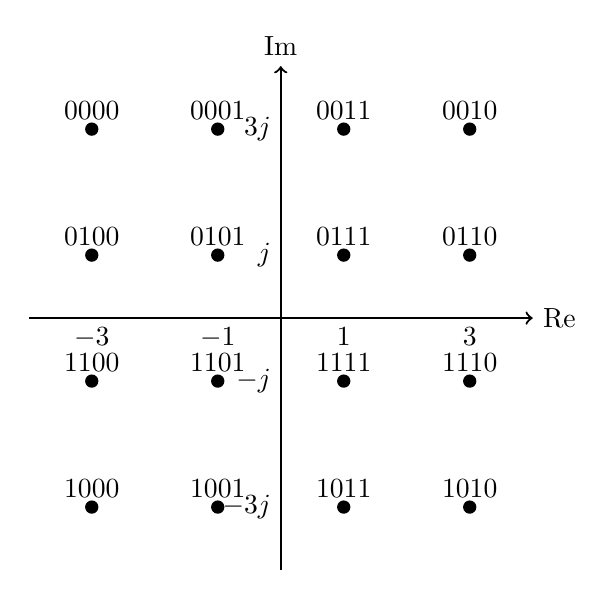
\begin{tikzpicture}[scale=0.8]
    \draw[->,thick] (-4,0) -- (4,0) node[right] {Re};
    \draw[->,thick] (0,-4) -- (0,4) node[above] {Im};
    \foreach \x/\y/\label in {
        -3/3/0000, -1/3/0001, 1/3/0011, 3/3/0010,
        -3/1/0100, -1/1/0101, 1/1/0111, 3/1/0110,
        -3/-1/1100, -1/-1/1101, 1/-1/1111, 3/-1/1110,
        -3/-3/1000, -1/-3/1001, 1/-3/1011, 3/-3/1010
    } {
        \fill (\x,\y) circle (3pt);
        \node[above] at (\x,\y) {\label};
    }
    \node at (-3,0) [below] {$-3$};
    \node at (-1,0) [below] {$-1$};
    \node at (1,0) [below] {$1$};
    \node at (3,0) [below] {$3$};
    \node at (0,3) [left] {$3j$};
    \node at (0,1) [left] {$j$};
    \node at (0,-1) [left] {$-j$};
    \node at (0,-3) [left] {$-3j$};
\end{tikzpicture}
\end{figure}

\subsection{发送信号经过多径信道传输}

信号经过多径信道的输出信号由下式表示
\begin{equation}
y[n] = \sum_{l=0}^{L-1} h_{l}[n]x[n-l] + w[n], n=0,...,K-1
\tag{43}
\end{equation}
式中 $L$ 为信道的多径数,$K$ 为传输信号的长度,$w[n]$ 为加性高斯白噪声,$h_{l}[n]$ 是信道参数。为了方便计算,将上式写成矩阵形式
\begin{equation}
Y = HX + W
\tag{44}
\end{equation}
其中,
\begin{equation}
Y = (y[0], y[1], ..., y[L-1], ..., y[n])^{T}
\tag{45}
\end{equation}

\begin{equation}
X = (x[0], x[1], \ldots, x[L-1], \ldots, x[n])^T
\tag{46}
\end{equation}

\begin{equation}
W = (w[0], w[1], \ldots, w[L-1], \ldots, w[n])^T
\tag{47}
\end{equation}

\begin{equation}
H = \begin{pmatrix}
h_0[0] & 0 & \cdots & 0 & \cdots & 0 \\
h_1[1] & h_0[1] & \cdots & 0 & \cdots & 0 \\
\vdots & \vdots & \ddots & \vdots & \ddots & \vdots \\
h_{L-1}[L-1] & h_{L-2}[L-1] & \cdots & h_0[L-1] & \cdots & 0 \\
\vdots & \vdots & \ddots & \vdots & \ddots & h_0[n-1] \\
0 & \cdots & h_{L-1}[n] & \cdots & h_0[n] & 0
\end{pmatrix}
\tag{48}
\end{equation}

信号经过多径衰落信道可以看作是信号与矩阵相乘。在仿真中,首先利用信道数据构建 $H$ 矩阵,与发送信号相乘即可得到信道输出信号,再叠加加性高斯白噪声即得到信道输出信号。

\subsubsection{接收信号检测}

接收端首先通过问题一建立的信道估计模型对信道进行估计,再利用相关检测算法将发送信号求出,如最小均方误差检测(MMSE)、迫零检测(ZF)、串行干扰删除(SIC)和最大似然检测(ML)等,最后进行判决将符号逆映射为比特。本文采用 SIC 检测算法对接收信号进行检测,SIC 算法流程如下

Step 1:从接收信号向量 $y_1$ 中分离出第一个判决统计量

\begin{equation}
r_1 = \omega \cdot y_1
\tag{49}
\end{equation}

其中 $\omega$ 是 $H^+$ 的第一行,$H^+$ 是信道特征矩阵 $H$ 的伪逆矩阵。

Step 2:由 $r_1$ 解调得出对发送符号 $s_1$ 的估值,以 $Q(\cdot)$ 表示量化判决。并假定判决无误 $s_1 = \hat{s}_1$:

\begin{equation}
\hat{s}_1 = Q(r_1)
\tag{50}
\end{equation}

Step 3:由检测得到的 $\hat{s}_1$ 重新调制得到相应接收信号,并从接收信号向量中抵消出,得到新的接收信号向量:

\begin{equation}
r_2 = y_1 - h_1 \hat{s}_1
\tag{51}
\end{equation}

其中,$h_1$ 是 $H$ 的第一列,更新后的接收信号向量除去了分离出的子信号的影响。

Step 4:返回第一步,从更新后的接收信号向量中分离第二个子信息流,重复以上步骤,直到依次分离译出整个接收信号向量。

\subsubsection{仿真结果}

(1) 接收信号星座图

图 14 画出了发送 20000 个比特时,接收端解调后的星座图。红色十字表示理想 16QAM 的星座图,蓝色表示接收端检测后的信号星座。由图可看出,接收信号大部分都能正确判决,只有少数星座点判决错误,说明了本文建立的信道估计模型的正确性。

\begin{figure}[h]
    \centering
    \includegraphics[width=\textwidth]{image1.png}
    \caption{接收信号星座图}
    \label{fig:14}
\end{figure}

(2) 误比特率曲线

\begin{figure}[h]
    \centering
    \includegraphics[width=\textwidth]{image2.png}
    \caption{误比特率曲线}
    \label{fig:15}
\end{figure}

为了直观地看出不同测试参数下信道估计的误比特率,图 \ref{fig:15} 画出了在不同测试参数和信道估计方法下,仿真得出的误比特率。由图可知,BEM 信道估计在测试速度为 $90\,\text{km/h}$ 时误比特率性能最好,在 $450\,\text{km/h}$ 测试时误比特率性能最差。在测试速度为 $180\,\text{km/h}$ 时,采用理想信道估计和 BEM 估计的误比特率性能基本一致,说明了 BEM 信道估计性能很好。在信噪比较低时 ($<20\,\text{dB}$),所有测试参数和信道估计方法的性能基本没有差别;在高信噪比时,不同方案的性能逐渐有所区别。

\section{模型评价与结论}

本文以泛化复指数基函数建立了基扩展模型,对附件给出的信道数据建立模型,通过选择不同的模型参数,可以在不同运动速度下都能获得较高的模型准确度。进一步研究发现,该模型在不同信道环境下具有良好的适应性和鲁棒性,能够有效捕捉信道的时变特性。此外,模型的参数优化过程也表明,通过合理的参数选择,可以显著提高模型的预测精度,从而为实际通信系统的信道建模和预测提供有力支持。

步分析了模型参数对模型准确度及复杂度的影响,模型准确度随基函数阶数增加指数增长,复杂度随阶数平方增长;训练样本取样间隔与模型准确度呈波动趋势。运动速度越大,模型准确度越小。

此外,基于 Clarke 模型,我们仿真了多径瑞利衰落信道,并用仿真信道验证了建立的模型。最后,通过 16QAM 调制,分析了该模型在实际通信系统的误码性能。

基扩展模型能够有效减少测试数据,从而提升无线通信系统的传输效率,但是,该模型的准确度严重依赖于基函数阶数,而模型复杂度是阶数的平方函数,所以减小模型复杂度是急待解决的问题。

\section{参考文献}

[1] Tomasz Hrycak, etc. Low Complexity Equalization for Doubly Selective Channels Modeled by a Basis Expansion, IEEE Trans. Signal Processing, 2010, 58(11):5706-5719.

[2] Saptarshi Das. Mathematical Methods for Wireless Channel Estimation and Equalization. Dissertation, University of Vienna, 2009.

[3] 吴伟凌等,移动通信原理(第 2 版),电子工业出版社,2009.1.

[4] 樊昌信等,通信原理(第 6 版),国防工业出版社,2013.8.

[5] Yahong R., etc. Improved Models for the Generation of Multiple Uncorrelated Rayleigh Fading Waveforms. IEEE Communications Letters, 2002,6(6):256-258.

[6] Tsatsanis M.K., Giannakis G.B. Equalization of rapidly fading channels: Self-recovering methods, IEEE Transactions on Communications, 44(5): 1996, 619-630.

[7] Leus G. On the estimation of rapidly time-varying channels, in Euro.Signal Process. Conf. (EUSIPCO)2004:2227”C2230.

[8] Zemen T., Mecklenbrauker C. F. "Time-variant channel estimation using discrete prolate spheroidal sequences" [J]. IEEE Transactions on Signal Processing, 53(9): 2005, 3597-3607.

[9] Giannakis G. B., Tepedelenlioglu C. Basis expansion models and diversity techniques for blind identification and equalization of time-varying channels, Proceedings of the IEEE, 86(10): 1998, 1969-1986.

[10] Idrees N. M., Haselmayr W., Schellander D., etc. Time variant channel estimation using a modified complex exponential basis expansion model in lte-ofdm systems, PIMRC 2010, 26-30 Sept. 2010.

[11] Robustness of Joint Bayesian Frequency Offset and Channel Estimation Based on Basis Expansion Models

[12] 周炯槃等,通信原理(第 3 版),北京邮电大学出版社,2008.8

\end{document}